\section{Probability}

\subsection{Terminology}

\begin{itemize}
	\item \textbf{Sample space} (denoted by $S$ or $\Omega$): A set of all possible outcomes of an experiment. For example, if an experiment involves rolling a die, its sample space is: $S=\{1, 2, 3, 4, 5, 6\}$. Another example: for an experiment involving drawing a set of five cards from a deck of $52$ cards, its sample space consists of all possible sets of five cards and its size is $|S|=\binom{52}{5}$.
	\item \textbf{Event} (denoted by $E$): An event is any subset of sample space: $E \subset S$. The event $E$ occurs when the outcome of the experiment is a member of $E$. In the dice example, the event would be something like ``number less than 4 appear on the roll'': $E=\{1, 2, 3\}$. In the poker example, $E$ would be a set of outcomes where there is a full house.
\end{itemize}

Consider two events $E_1$ and $E_2$. Union of events $E_1 \cup E_2$ consists of outcomes that are either in $E_1$ or $E_2$ or both. Intersection $E_1 \cap E_2$ consists of outcomes which are both in $E_1$ and $E_2$. Events are said to be disjoint (or mutually exclusive) iff $E_1 \cap E_2 = \emptyset$. The complement of the event $E$ is denoted by $E^c$. It is the set of outcomes in $S$ that is not in $E$. \\

Events follow distributive laws: $E_1 \cap (E_2 \cup E_3) = (E_1 \cap E_2) \cup (E_1 \cap E_3)$ and $E_1 \cup (E_2 \cap E_3) = (E_1 \cup E_2) \cap (E_1 \cup E_3)$. \\

Revisiting the dice example, let $E_1$ be the event when a number less than 4 appears on the roll: $E_1=\{1, 2, 3\}$ and let $E_2$ be the event when an odd number appears on the roll: $E_2=\{1, 3, 5\}$. Union of the these events is: $E_1 \cup E_2 = \{1, 2, 3, 5\}$ and the intersection is: $E_1 \cap E_2 = \{1, 3\}$. The complement of $E_1$ is $E_1^c=\{4, 5, 6\}$.

\begin{figure}[H]
	\centering
	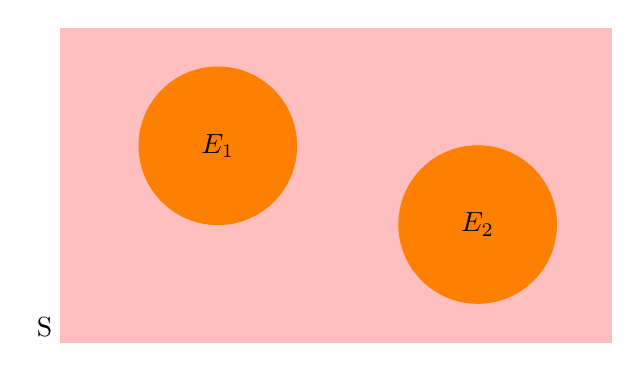
\begin{tikzpicture}
		\fill[pink] (0,0) rectangle (7,4);
		\draw[orange,fill=orange] (2,2.5) circle (1);
		\draw[orange,fill=orange] (5.3,1.5) circle (1);
		\node at (-0.2,0.2) {S};
		\node at (2,2.5) {$E_1$};
		\node at (5.3,1.5) {$E_2$};
	\end{tikzpicture}
	\caption{Cartoon illustrating sample space $S$ and disjoint events $E_1$ and $E_2$}
\end{figure}

\subsection{Defining Probability}

When repeating the experiment with sample space $S$ $n$ times, let $N_n (E)$ be the number of times $E$ occurs. Probability $P(E)$ of the event $E$ is defined as:

$$\displaystyle P(E) = \lim_{n \to \infty} \frac{N_n (E)}{n}$$

More formally, Probability is defined as a measure which is a function $P$ that assigns to each $E$ as a number and satisfies the following axioms:

\begin{enumerate}[i]
	\item $0 \le P(E) \le 1$ for all $E$
	\item $P(S)=1$ and $P(\emptyset)=0$
	\item For disjoint events $E_1, E_2, ..., E_N$: $\displaystyle P\left( \bigcup_{n=1}^N E_n \right)=\sum_{n=1}^N P(E_n)$
\end{enumerate}

If $S$ is finite (which happens often), we care about finite sequence of events only. The tuple $(S,\mathcal{F},P)$ constructs a probability space where $\mathcal{F}=\mathcal{P}(S)$\footnote{$\mathcal{P}$ is power set} is an event space which consists of all possible outcomes in the sample space $S$. Each event is often equally likely but not always (see the coin-flipping example below for instance). When events are equally likely, $P(E)=\frac{|E|}{|S|}$.

\begin{texample}
	A coin is tossed until either two Tails appear successively, or until the fifth toss, whichever comes first. The outcome is the resulting sequence of coins. \\
	
	There are $20$ possible outcomes which is described by the following sample space
	
	\begin{align*}
		S&=\{(HHHHH), (THHHH), (HTHHH), (HHTHH), \\
		&\quad (HHHTH), (HHHHT), (TT), (HTT), (HHTT), (THTT), \\
		&\quad (HHHTT), (THHHT), (HTHHT), (HHTHT), (HHTTH), \\
		&\quad (THHTH), (HTHTH), (HTTHH), (THTHH), (TTHHH)\}
	\end{align*}
	
	Outcomes in this sample space is not equally likely. For example $P(\{(TT)\})=\frac{1}{4}$ and $P(\{(HTT)\})=\frac{1}{8}$. The total probability is
	
	\begin{align*}
		P(S)&=P(\{(TT)\})+P(\{(HTT)\}) \\
		&\quad+2 P(\{(HHTT)\})+16  P(\{(HHHTT)\}) \\
		&=\frac{1}{4}+\frac{1}{8}+2\frac{1}{16}+16\frac{1}{32} \\
		&=1
	\end{align*}
	
	as expected.
\end{texample}

\begin{texample}
	In the game of poker, find $P(\text{four of a kind})$, $P(\text{full house})$, $P(\text{a pair})$, $P(\text{two pairs})$, and $P(\text{straight})$. \\
	
	As mentioned before, the size of the sample space is $|S|=\binom{52}{5}=2598960$. We need to find how many possible sets of four-of-a-kind $|E|$. There are $13$ different values for the first four cards (there are four suit options and each of the four cards takes a distinct suit but we don't count permutations here) and once the four cards are out, there are $48$ ($12$ choices for value and $4$ choices for suit) options for the last card. So $|E|=13(48)=624$. Therefore, $P(\text{four of kind})=\frac{|E|}{|S|}=0.00024$. \\
	
	There are $13$ possible card values for the first three cards. They can take any suit and there are $\binom{4}{3}=4$ different suit combinations for the first three cards. For the remaining two cards, there are $12$ possible values and $\binom{4}{2}=6$ different suit combinations. So $|E|=3744$ and the probability is therefore $P(\text{full house})=0.00144$. \\
	
	There are $\binom{13}{1}$ ways to pick a value for a pair. There are $\binom{4}{2}$ different suit combinations for a pair. There are $\binom{12}{3}$ ways to pick $3$ distinct values for the rest of the $3$ cards and each card has $\binom{4}{1}$ different suit combinations. The answer is $\frac{\binom{13}{1}\binom{4}{2}\binom{12}{3}\binom{4}{1}^3}{\binom{52}{5}}=0.4226$. \\
	
	There are $\binom{13}{2}$ ways to pick values for two pairs. There are $\binom{4}{2}$ different suit combinations for each pair. There are $\binom{11}{1}$ ways to pick a distinct value for the last card and has $\binom{4}{1}$ different suit combinations. The answer is $\frac{\binom{13}{2}\binom{4}{2}^2\binom{11}{1}\binom{4}{1}}{\binom{52}{5}}=0.04754$. \\
	
	There are 10 possible values for the initial card. There are 4 suit options for each of the five cards, so there are $4^5$ suit combinations but to exclude straight flushes we subtract it by 4. This gives $|E|=10(4^5-4)=10200$, so $P(\text{straight})=0.00392$.
\end{texample}

\begin{texample}
	There are $7$ marbles in a bag, $4$ red and $3$ blue. You draw marbles one at a time without replacement. What is the probability that the fifth marble is blue? \\
	
	One way to do this problem is to try labelling each marble from $1$ to $7$ which represents the order of drawing out. So the probability that the blue marble gets $5$ is $\frac37$.
\end{texample}

\begin{texample}
	You roll five dice, find probabilities for (a) one pair ($aabcd$) (b) two pairs ($aabbc$) (c) full house ($aaabb$). \\
	
	(a) There are $\binom{6}{4}$ ways to pick values for the set $\{a, b, c, d\}$. There are $\frac{5!}{2!}$ ways to arrange $aabcd$. There are $4$ ways to select the value of a pair from the set $\{a, b, c, d\}$. There are $6^5$ permutations in total. The final answer is $\frac{\binom{6}{4}\frac{5!}{2!}4}{6^5}=0.46296$. \\
	
	(b) Caring about order, there are $\binom{6}{2}$ ways to pick values for the pairs $\{a, b\}$ and $\binom{4}{1}$ ways to pick the value of $c$. There are $\frac{5!}{2!2!}$ ways to arrange $aabbc$. There are $6^5$ permutations in total. The final answer is $\frac{\binom{6}{2}\binom{4}{1}\frac{5!}{2!2!}}{6^5}=0.23148$. \\
	
	(c) There are $\binom{6}{1}$ ways to pick values for $a$ and $\binom{5}{1}$ ways to pick values for $b$. There are $\frac{5!}{3!2!}$ ways to arrange $aaabb$. The final answer is $\frac{\binom{6}{1}\binom{5}{1}\frac{5!}{3!2!}}{6^5}=0.03858$.
\end{texample}

Note on counting: $\binom{6}{1}\binom{5}{1}$ is not equal to $\binom{6}{2}$. The former is used if order matters otherwise the latter is used. In fact, $\binom{6}{1}\binom{5}{1}=2\binom{6}{2}={}_6P_2$. Imagine you have a bag of marbles labelled $1, 2, \dots, 6$, $\binom{6}{2}$ counts the number of two marble combinations while $\binom{6}{1}\binom{5}{1}$ counts the number of ways to pick the first marble and paint it red then pick the second marble.

\begin{texample}
	A box contains $15$ lego bricks: $3$ red bricks, $3$ green bricks, $3$ blue bricks, $3$ yellow bricks and $3$ purple bricks. You draw 5 bricks from the box at random without replacement. What is the probability of getting $5$ distinct colours? \\
	
	There are $15\cdot14\cdot13\cdot12\cdot11$ different ordered selections ($15$ options for the first brick, $14$ options for the second brick and so on). Now, there are $15$ options for the first brick which can be in any colour. Then there are $12$ options for the second brick (we exclude all bricks with the same colour as the first brick). There are $9$ options for the third brick (we exclude all bricks with the same colour as the first and second bricks) and so on. The probability is
	
	\[\frac{15}{15}\frac{12}{14}\frac{9}{13}\frac{6}{12}\frac{3}{11}=\frac{81}{1001}\]
\end{texample}

\begin{texample}
	You have $13$ cards, $6$ red ($R$) and $7$ black ($B$). You shuffle them and place them face up in two rows. The top row has $5$ cards, the bottom row $8$. If you do this many times, what number of red cards will the top row have most often? \\
	
	The total number of arrangements is $\frac{13!}{6!7!}=1716$. \\
	
	To determine the most likely number of red cards, we count the number of arrangements when the top row has $0, 1, 2, 3, 4, 5$ red cards. For example, to count the number of arrangements for the top row with $2$ red cards, $\binom{5}{2}=\frac{5!}{2!3!}=10$. To get the total number of arrangements we multiply the results, for example, the total number of arrangements with $3$ red cards at the top is $10(56)=560$. After that, we calculate probabilities and compare.
	
	\begin{center}
		\footnotesize
		\begin{tabular}{l|l|l|l|l|l|l}
			\text{no. red at top} & 0 & 1 & 2 & 3 & 4 & 5 \\
			\hline
			\text{no. arrangements for top} & 1 & 5 & 10 & 10 & 5 & 1 \\
			\hline
			\text{no. red at bottom} & 6 & 5 & 4 & 3 & 2 & 1 \\
			\hline
			\text{no. arrangements for bottom} & 28 & 56 & 70 & 56 & 28 & 8 \\
			\hline
			\text{total no. of arrangements} & 28 & 280 & 700 & 560 & 140 & 8 \\
			\hline
			\text{probability} & 0.016 & 0.163 & 0.408 & 0.326 & 0.082 & 0.005
		\end{tabular}
	\end{center}
	
	From the table, we see that the top row will most likely have $2$ red cards. \\
	
	Also notice that $28+280+700+560+140+8=1716$. \\
	
	If we were to compute the average number of red cards in the top row, we use the following relation: $\sum_{n=0}^5 nP_n$ where $P_n$ is the probability of getting $n$ red cards in the top row. This gives:
	
	$$0(0.016) + 1(0.163) + 2(0.408) + 3(0.326) + 4(0.082) + 5(0.005)=2.31$$
	
	This playing card example has applications in statistical mechanics for modelling two-state systems.
\end{texample}

\begin{texample}
	You have a standard deck of $52$ cards which consists of $26$ red cards and $26$ black cards. The deck is shuffled well, what is the probability that the first five cards contain $3$ red cards and $2$ black cards? What is the probability if the deck is large enough? \\
	
	We count the number of ways to draw $3$ red cards from the set of $26$ red cards: $\binom{26}{3}$ and the number of ways to draw $2$ black cards from the set of $26$ black cards: $\binom{26}{2}$. Then multiply the result and divide it by the number of ways to draw $5$ cards from the deck: $\binom{52}{5}$. This gives $P(3R,2B)=\frac{\binom{26}{3}\binom{26}{2}}{\binom{52}{5}}$. \\
	
	Alternative approach: Count the number of combinations of a $5$ card hand that contains $3$ red and $2$ black: $\binom{5}{3}$. Then count the number of ways to rearrange the remaining cards in the deck: $\binom{52-5}{26-3}$. Finally count the number of ways to arrange the deck: $\binom{52}{26}$. This gives $P(3R,2B)=\frac{\binom{5}{3}\binom{52-5}{26-3}}{\binom{52}{26}}$. \\
	
	To approximate the probability when the deck is large, we rewrite things a bit:
	
	\begin{align*}
		P(3R,2B)&=\frac{\binom{26}{3}\binom{26}{2}}{\binom{52}{5}} \\
		&=\frac{\frac{26!}{3!23!}\frac{26!}{2!24!}}{\frac{52!}{5!47!}} \\
		&=\frac{5!}{3!2!}\frac{\frac{47!}{23!24!}}{\frac{52!}{26!26!}} \\
		&=\frac{5!}{3!2!}\frac{(52-5)!26!26!}{52!(26-3)!(26-2)!} \\
		&=\frac{5!}{3!2!}\frac{26(26-1)(26-2)26(26-1)}{52(52-1)(52-2)(52-3)(52-4)} \\
		&\approx \frac{5!}{3!2!}\frac{26^5}{56^5} \\
		&\approx \frac{5!}{3!2!}\frac{1}{2^5}
	\end{align*}
	
	We conclude that the suitable approximation is $\frac{\binom{5}{3}}{2^5}$. This gets better when the deck is larger. \\
	
	This example illustrates the concept of heat bath. The larger the deck is, taking out a few cards will have almost no effect on the probability.
\end{texample}

\subsection{Useful Probability Relations}

Probability has the following useful properties:

\begin{enumerate}[i]
	\item For a single event $E$, $P(S)=P(E)+P(E^c)=1$. $E$ and $E^c$ is always disjoint.
	\begin{figure}[H]
		\centering
		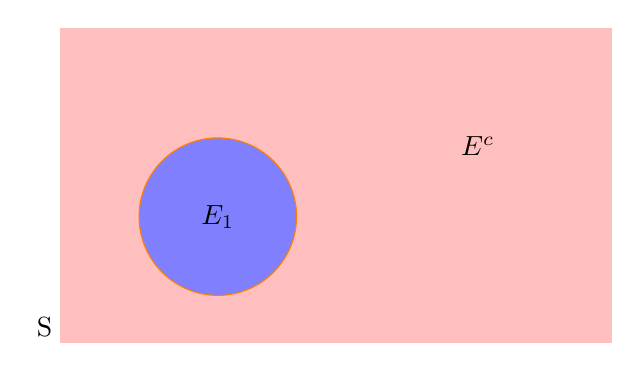
\begin{tikzpicture}
			\fill[pink] (0,0) rectangle (7,4);
			\draw[orange,fill=blue!50] (2,1.6) circle (1);
			\node at (-0.2,0.2) {S};
			\node at (2,1.6) {$E_1$};
			\node at (5.3,2.5) {$E^c$};
		\end{tikzpicture}
		\caption{Event $E$ and its complement $E^c$}
	\end{figure}
	\item For two non-disjoint events $E_1$ and $E_2$, probability can be calculated using inclusion-exclusion principle: $P(E_1 \cup E_2) = P(E_1) + P(E_2) - P(E_1 \cap E_2)$.
	\def\firstcircle{(0,0) circle (1.8cm)}
	\def\secondcircle{(0:2cm) circle (1.8cm)}
	\begin{figure}[H]
		\centering
		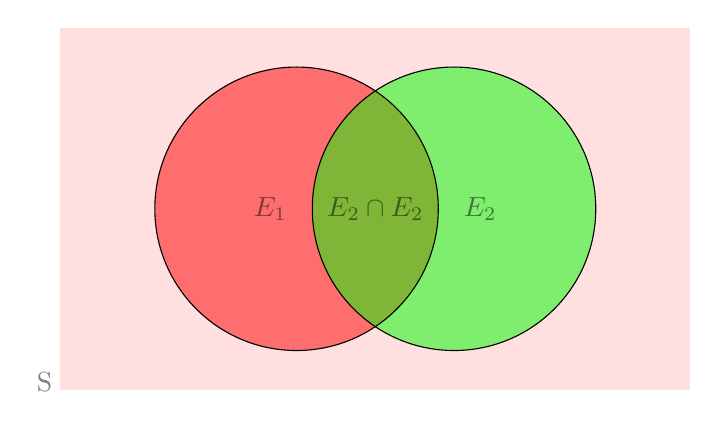
\begin{tikzpicture}
			\begin{scope}[shift={(3cm,-5cm)}, fill opacity=0.5]
				\fill[pink] (-3,-2.3) rectangle (5,2.3);
				\fill[red] \firstcircle;
				\fill[green] \secondcircle;
				\draw \firstcircle node [left] {$E_1$};
				\draw \secondcircle node [right] {$E_2$};
				\node at (0:1cm) {$E_2 \cap E_2$};
				\node at (-3.2,-2.2) {S};
			\end{scope}
		\end{tikzpicture}
		\caption{Cartoon illustrating non-disjoint events $E_1$ and $E_2$}
	\end{figure}
	For disjoint events, $P(E_1 \cap E_2)$ = 0 since $E_1 \cap E_2 = \emptyset$. \\
	
	For three events, it becomes:
	
	\begin{align*}
		P(E_1 \cup E_2 \cup E_3) &= P(E_1) + P(E_2) + P(E_3) \\
		&\phantom{-} - P(E_1 \cap E_2) - P(E_2 \cap E_3) - P(E_1 \cap E_3) \\
		&\phantom{-} + P(E_1 \cap E_2 \cap E_3)
	\end{align*}
	
	\begin{figure}[H]
		\centering
		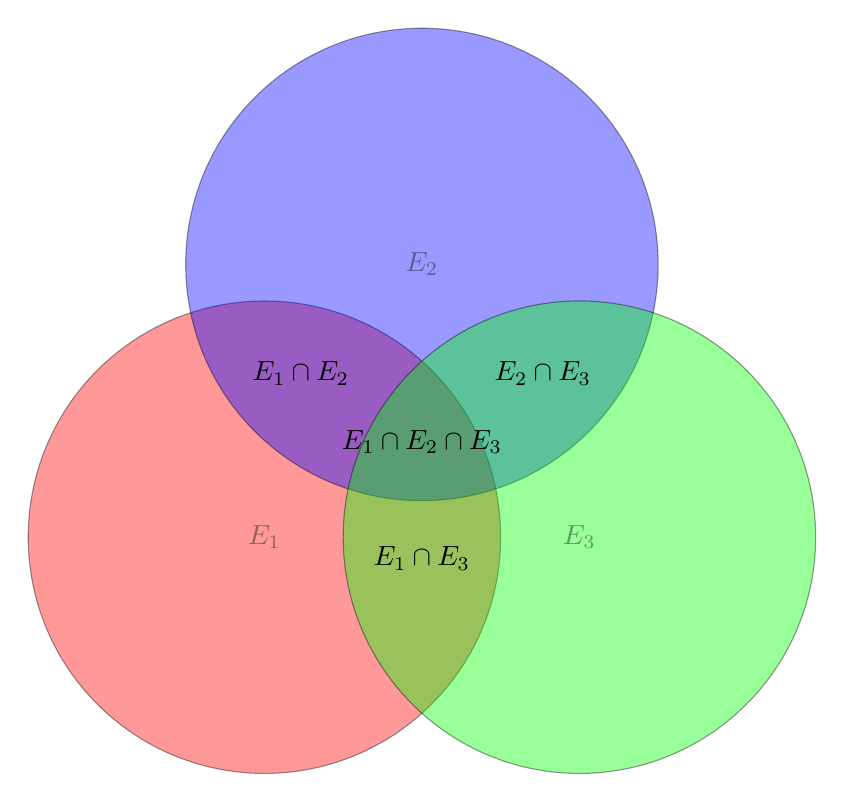
\begin{tikzpicture}
			\tikzset{venn circle/.style={draw,circle,minimum width=6cm,fill=#1,opacity=0.4}}
			\node [venn circle = red] (A) at (0,0) {$E_1$};
			\node [venn circle = blue] (B) at (60:4cm) {$E_2$};
			\node [venn circle = green] (C) at (0:4cm) {$E_3$};
			\node[left] at (barycentric cs:A=1/2,B=3/4 ) {$E_1 \cap E_2$}; 
			\node[below] at (barycentric cs:A=1/2,C=1/2 ) {$E_1 \cap E_3$};   
			\node[right] at (barycentric cs:B=3/4,C=1/2 ) {$E_2 \cap E_3$};   
			\node[below] at (barycentric cs:A=1/3,B=1/2,C=1/3 ){$E_1 \cap E_2 \cap E_3$};
		\end{tikzpicture}  
		\caption{Three non-disjoint events $E_1$, $E_2$ and $E_3$}
	\end{figure}
	
	For more than three events, the inclusion-exclusion principle can be generalized to:
	
	\begin{align*}
		P\left( \bigcup_{n=1}^N E_n \right) &= \sum_{i} P(E_i) \\
		&\phantom{-} - \sum_{i<j} P(E_i \cap E_j) \\
		&\phantom{-} + \sum_{i<j<k} P(E_i \cap E_j \cap E_k) \\
		&\phantom{-} - \sum_{i<j<k<l} P(E_i \cap E_j \cap E_k \cap E_l) + \cdots + (-1)^{n-1} P\left( \bigcap_{n=1}^N E_n \right)
	\end{align*}
\end{enumerate}

\begin{texample}
	Birthday problem: There are $n$ people in the room, what is the probability that at least two of them share the same birthday? \\
	
	The sample space $S$ for this experiment consists of sequences of $n$ birthdays: $(B_1, B_2, \dots, B_n) \in S$. The size of the sample space is $|S|=365^n$, ignoring leap years. The event $E$ is the set of sequences that contains at least two matching birthdays, like for example $E=\{\dots (09/11, \dots, 09/11) \dots\}$. \\
	
	We first calculate the probability that all $n$ birthdays are different. This is the complement of the event $E$, denoted by $E^c$. There are $365$ unique choices for the first person's birthday and this leaves with $364$ choices for the second person's birthday and so on. The probability is:
	
	$$ P(\text{all different})=\frac{|E^c|}{|S|}=\frac{365 \cdot 364 \cdot 363 \cdots (365-n+1)}{365^n}=\frac{{}_{365} \mathrm{P}_n}{365^n}$$
	
	The probability that at least two people share the same birthday is therefore:
	
	$$P(\text{at least two same bday})=1-P(\text{all different})=1-\frac{{}_{365} \mathrm{P}_n}{365^n}$$
	
	To illustrate the result, suppose $n=23$, the probability is $P(\text{at least two same bday})=0.5073$.
\end{texample}

\begin{texample}
	You flip two coins. Find the probability that either the first or the second coin fall heads. \\
	
	The possible outcomes $S$ for this experiment are: $S=\{(H, H), (H, T), (T, H), (T,T)\}$. Let $E_1$ be the event that the first coin falls heads: $E_1=\{(H, H), (H, T)\}$ and $E_2$ be the event that the second
	coin falls heads: $E_2=\{(H, H), (T, H)\}$. By the inclusion-exclusion principle:
	
	\begin{align*}
		P(E_1 \cup E_2) &= P(E_1) + P(E_2) - P(E_1 \cap E_2) \\
		&= \frac{1}{2}+\frac{1}{2}-\frac{1}{4}=\frac{3}{4}
	\end{align*}
	
	It can be computed directly as well: $P(E_1 \cup E_2)=P(\{(H, H), (H, T), (T, H)\})=\frac{3}{4}$.
\end{texample}

\begin{texample}
	Find the probability that the random permutation of $1112345$ does not have adjacent identical digits. \\
	
	We label $1$s to distinguish them: $1_a 1_b 1_c 2345$. The sample space $S$ is all permutations of $1_a 1_b 1_c 2345$ and the size is $|S|=7!=5040$ (remember that $1$s are distinct from each other!). Let $E_{ab}$, $E_{bc}$, $E_{ac}$ denote events where ``$1_a$ and $1_b$ are adjacent,'' ``$1_b$ and $1_c$ are adjacent'' and ``$1_a$ and $1_c$ are adjacent'' respectively. The probability that there are no adjacent ones can be calculated using the inclusion-exclusion principle:
	
	\begin{align*}
		P(\text{no adjacent 1s}) &= 1 - P(E_{ab} \text{ or } E_{bc} \text{ or } E_{ac}) \\
		&= 1 - P(E_{ab}) - P(E_{bc}) - P(E_{ac}) \\
		& \quad + P(E_{ab} \text{ and } E_{bc}) + P(E_{ab} \text{ and } E_{bc})  \\
		& \quad + P(E_{ac} \text{ and } E_{bc}) \\
		& \quad - P(E_{ab} \text{ and } E_{bc} \text{ and } E_{ac})
	\end{align*}
	
	By symmetry and the fact that $1_a, 1_b, 1_c$ cannot *all* be adjacent to each other:
	
	$$P(\text{no adjacent 1s}) = 1 - 3 P(E_{ab}) + 3 P(E_{ab} \text{ and } E_{bc})$$
	
	$P(E_{ab}) = \frac{2 (6!)}{7!} = \frac27$: if $1_a$ and $1_b$ are adjacent, we can treat them as one symbol $[1_a 1_b]$, so there are $6!$ ways to order the $6$ symbols we now have, and then $2$ ways to choose the order of $1_a$ and $1_b$. Similarly, $P(E_{ab} \text{ and } E_{bc})$ can be calculated by treating $[1_a 1_b 1_c]$ as a symbol. There are two valid permutations where $[1_a 1_b]$ and $[1_b 1_c]$ combinations exist, namely $[1_a 1_b 1_c]$ and $[1_c 1_b 1_a]$. This gives $\frac{2 (5!)}{7!}=\frac{1}{21}$. \\
	
	The final answer is:
	
	$$P(\text{no adjacent 1s}) = 1 - 3 \frac27 + 3 \frac{1}{21} = \frac27$$
\end{texample}

\begin{texample}
	$n$ people put their names in a hat. The hat is shaken and $n$ people draw names out of the hat (secret Santa). What is the probability that nobody gets their own name? \\
	
	We label each person from $1$ to $n$. The sample space $S$ is all permutations of $\{1, 2, \dots, n\}$ and its size is $|S|=n!$. Let $E_i$ denote an event where person $i$ gets their own name: $E_i=\{ \text{permutations where person $i$ gets their own name.} \}$. We first calculate $P(E_1 \cup E_2 \cup \cdots \cup E_n)$. \\
	
	First, we calculate $P(E_i)$. The number of events where person $1$ gets his own name $|E_1|$ can be calculated by placing person $1$ on position $1$ from the start and counting the number of ways to arrange the remaining $n-1$ people on positions $2, 3, \dots n$ which is $(n-1)!$. The probability that person $1$ gets his own name is $P(E_1)=\frac{(n-1)!}{n!}=\frac{1}{n}$. By symmetry, $P(E_i)=P(E_1)$ for $i=1, 2, \dots n$. \\
	
	Next we calculate $P(E_i \cap E_j)$. $|E_1 \cap E_2|$ is the number of events where both person $1$ and person $2$ gets their own names. The calculation process is similar: place persons $1$ and $2$ at positions $1$ and $2$ respectively and calculate the number of ways to arrange the remaining $n-2$ people on positions $3, \dots n$ which is $(n-2)!$. So, $P(E_1 \cap E_2)=\frac{(n-2)!}{n!}$ and by symmetry, $P(E_i \cap E_j)=P(E_1 \cap E_2)$ for any $i<j$. There are $\binom{n}{2}$ pairs of $i,j$. \\
	
	We can generalize that the probability that $k$ people get their own names is $\frac{(n-k)!}{n!}$ and there are $\binom{n}{k}$ combinations of $k$ people. Now by the inclusion-exclusion principle:
	
	\begin{align*}
		P\left( \bigcup_{n=1}^N E_n \right) &= n P(E_1) - \binom{n}{2} P(E_1 \cap E_2) + \binom{n}{3} P(E_1 \cap E_2 \cap E_3) \\
		&\phantom{-} + \cdots \pm (-1)^{n-1} P\left( \bigcap_{n=1}^N E_n \right) \\
		&= n\frac{1}{n} - \binom{n}{2}\frac{(n-2)!}{n!} + \binom{n}{3}\frac{(n-3)!}{n!} - \dots + \frac{(-1)^{n-1}}{n!} \\
		&= \sum_{k=1}^N (-1)^{k-1}\binom{n}{k}\frac{(n-k)!}{n!} \\
		&= \sum_{k=1}^N (-1)^{k-1} \frac{1}{k!} = 1-e^{-1}
	\end{align*}
	
	Therefore the probability that nobody draws their own name is $1-(1-e^{-1})=e^{-1}=0.368$.
\end{texample}

\subsection{Conditional Probability and Independent Events}

Suppose there are two events $E$ and $F$. Assume that $P(F)>0$. The probability that $E$ happens given that $F$ happened is denoted by $P(E|F)$. Imagine $E$ and $F$ lie on s sample space $S$.

\def\firstcircle{(0,0) circle (1.8cm)}
\def\secondcircle{(0:2cm) circle (1.8cm)}
\begin{figure}[H]
	\centering
	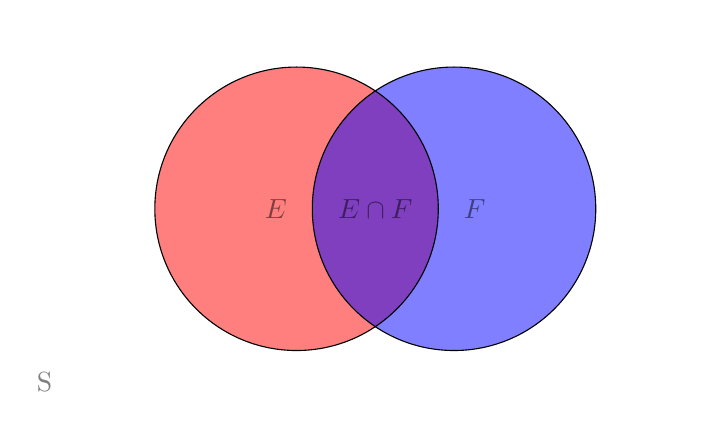
\begin{tikzpicture}
		\begin{scope}[shift={(3cm,-5cm)}, fill opacity=0.5]
			\fill[white] (-3,-2.3) rectangle (5,2.3);
			\fill[red] \firstcircle;
			\fill[blue] \secondcircle;
			\draw \firstcircle node [left] {$E$};
			\draw \secondcircle node [right] {$F$};
			\node at (0:1cm) {$E \cap F$};
			\node at (-3.2,-2.2) {S};
		\end{scope}
	\end{tikzpicture}
	\caption{Events $E$ and $F$}
\end{figure}

Recall that the probability of $P(E)$ is proportional to the probability of the sample space $P(S)=1$. When event $F$ happens, $F$ will become a new sample space as illustrated below.

\begin{figure}[H]
	\centering
	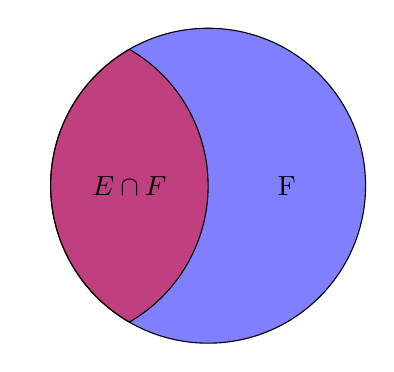
\begin{tikzpicture}
		\draw[fill=blue, fill opacity=0.5] (0,0) circle (2);
		\draw[fill=red, fill opacity=0.5] (120:2)
		arc[start angle=60, end angle=-60, radius=2]
		arc[start angle=240, end angle=120, radius=2];
		\node at (180:1) {$E \cap F$};
		\node at (0:1) {F};
	\end{tikzpicture}
	\caption{New sample space $F$}
\end{figure}

With this new sample space, we can be sure that everything happens on $F$. $E|F$ indicates both events $E$ and $F$ happen, so we have $E \cap F$ lie in $F$. We can now define $P(E|F)$ as a ratio of $E \cap F$ to $F$, assuming that every outcome in $F$ is equally likely:

$$P(E|F)=\frac{|E \cap F|}{|F|}$$

Dividing both numerator and denominator by $|S|$ gives:

$$P(E|F)=\frac{\frac{|E \cap F|}{|S|}}{\frac{|F|}{|S|}}=\frac{P(E \cap F)}{P(F)}$$

We derived the formula for conditional probability. It satisfies all probability axioms. As a corollary, this formula is also written in this way:

$$P(E \cap F)=P(F)P(E|F)$$

This is intuitive: ``probability for both $E$ and $F$ happen is the probability that $F$ happens times the probability that $E$ happens \textit{given} that $F$ happened.'' \\

Two events $E$ and $F$ are independent if finding out one event does not affect the probability of another, that is $P(E|F)=P(E)$. This means uncovering the existence of $F$ does not affect the probability of $E$ happening. We can test whether events are independent or not using the below relation:

$$P(E \cap F)=P(F)P(E)$$

Note that disjoint and independent are two different things. Events being disjoint means they are mutually exclusive. Here are some examples of (non-)disjoint and (in)dependent events.

\begin{enumerate}
	\item \textbf{Disjoint but dependent events}
	
	Consider an experiment of rolling a die. Define events $E$ to be ``roll $3$'' and $F$ to be ``roll $4$.'' These events are disjoint because you can't roll both $3$ and $4$ at the same time using a single dice and this makes $P(E \cap F)=0$. It implies that events are not independent (ie. dependent) because of $P(E \cap F) \ne P(E)P(F)$. Also since $P(E \cap F)=0$, $P(E|F)=0$ which makes sense in this context. \\ 
	
	We can conclude that disjoint events cannot be independent. There are exceptions, for example, consider the game of darts. Define events $E$ "dart land on target" and $F$ "dart land on the edge of the board." $P(E\cap F)=0$ since a dart land at both places same time but $P(E)=0$ and $P(F)=0$ since there are infinitely many points but it is still possible to land on one of them. Events $E$ and $F$ are disjoint but independent events.
	\item \textbf{Independent but not disjoint events}
	
	Consider the dice experiment again but with two dice this time. Define events $E$ "the sum of the face values is $7$" and $F$ the face value of the first die is $2$. They are not disjoint because there is a possible outcome where the sum of the face value is $7$ and the face value of the first die is $2$: $\{2, 5\}$. $E$ and $F$ are independent because $P(E\cap F)=\frac{1}{36}$ and $P(E)P(F)=\frac{1}{36}$. But if we redefine $E$ to be ``the sum of the face values is $6$,'' the events will become dependent because the probability depends on whether we rolled $6$ on the first roll or not (we must roll numbers $1$ to $5$ to get some chance that the face values totalling $6$).
	\item \textbf{Dependent but not disjoint events}
	
	We discussed an example of dependent but not disjoint events previously but here is another one: In an experiment where you draw two balls from a bag containing $5$ red balls and $3$ green balls without replacement, define events $E$ "draw a red ball on the first draw" and $F$ "two balls are red." They are not disjoint because there is an outcome where $E$ and $F$ happen at the same time: $\{R, R\}$. They are dependent (ie. not independent) because $P(E\cap F)=P(E)P(F|E)=\frac58 \frac47=\frac{5}{14}$ and $P(E)P(F)=\frac58 \frac{5}{14}=\frac{25}{112}$.
\end{enumerate}

For more than two events, events $E_1, E_2, \dots, E_n$ are independent iff

$$P\left(\bigcup_i^k E_{i'} \right) = \prod_i^k P(E_{i'})$$

for every subset $E_{1'}, E_{2'}, \dots. E_{k'}$ of size $k\le n$. \\

If events $A,B,C,D$ are dependent:

$$P(A\cap B\cap C\cap D) = P(A)P(B|A)P(C|A\cap B)P(D|A\cap B\cap C)$$

\begin{texample}
	You draw two cards from a standard deck. Define events $E$ ``draw hearts as the first card'' and $F$ ``draw hearts as the second card.'' Find $P(\text{draw two hearts})$. \\
	
	We have $P(E)=P(F)=\frac{13}{52}$ and
	
	$$P(E \cap F)=P(E)P(F|E)=\frac{13}{52}\frac{12}{51}=\frac{1}{17}$$
	
	or alternatively, $P(E \cap F)=\frac{{13 \choose 2}}{{52 \choose 2}}=\frac{1}{17}$. \\
	
	The events $E$ and $F$ are dependent because $P(E \cap F) \ne P(E)P(F)$.
\end{texample}

\begin{texample}
	You draw a card from a standard deck. Define events $E$ ``draw red card'' and $F$ ``draw ace.'' Find $P(\text{red ace})$. \\
	
	We find that $P(E)=\frac{1}{2}$ and $P(F)=\frac{4}{52}=\frac{1}{13}$. To find $P(\text{red ace})$, we calculate $P(E \cap F)$:
	
	$$P(E \cap F)=P(F)P(E|F)=\frac{1}{13}\frac{1}{2}=\frac{1}{26}$$
	
	Notice that $P(E|F)=P(E)$ which makes events $E$ and $F$ independent.
\end{texample}

\begin{texample}
	You toss two coins. Define events $E$ ``first coin heads,'' $F$ ``second coin heads'' and $G$ ``both heads or both tails.'' Are these three events mutually independent? \\
	
	The sample space is $S=\{HH, HT, TH, TT\}$. We have $P(E)=\frac12$, $P(F)=\frac12$ and $P(G)=\frac12$. Any of these two events are independent, for example, $P(E\cap F)=\frac14$ which is equal to $P(E)P(F)=\frac12\frac12=\frac14$. However, $P(E \cap F \cap G)=\frac14$ which is not equal to $P(E)P(F)P(G)=\frac18$, so the three events combined are not independent.
\end{texample}

\begin{texample}
	You roll two dice blindfolded. You are told that the sum is not greater than $3$, what is the probability that both dice have the same face value? \\
	
	Let $E$ be the event when both dice have the same face value and $F$ be the event when the sum is not greater than $3$. Since they both share the $\{1, 1\}$ outcome, the events are not disjoint. \\
	
	We wish to calculate $P(E|F)$. We have $P(E)=\frac{6}{36}=\frac16$ and $P(F)=\frac{3}{36}=\frac{1}{12}$ (the possible outcomes are $\{1, 1\}$, $\{1, 2\}$ and $\{2, 1\}$). The probability to get both events is $P(E \cap F)=\frac{1}{36}$. This makes events $E$ and $F$ dependent since $P(E \cap F) \ne P(E)P(F)$. Therefore $P(E|F)$ is given by:
	
	$$P(E|F)=\frac{P(E \cap F)}{P(F)}=\frac{\frac{1}{36}}{\frac{1}{12}}=\frac{1}{3}$$
\end{texample}

\subsection{Law of Total Probability}

Let $F_1, F_2, \dots, F_n$ denote partitions of sample space $S$ in such way that

$$S=\bigcup_i^n F_i$$

There is also an event $E$ in $S$. We want to find the relationship between $E$ and $F_1, F_2, \dots, F_n$.

\begin{figure}[H]
	\centering
	\includegraphics[width=130mm]{2.png}
	\caption{Partitions of $S$}
\end{figure}

From the diagram, we see that $E$ is expressed as disjoint unions (coloured regions) of $E \cap F_i$, so

$$P(E)=\sum_i P(E \cap F_i) = \sum_i P(F_i) P(E|F_i)$$

This is the law of total probability. It expresses $P(E)$ in terms of weighted averages of $P(E|F_i)$s. For two events $E$ and $F$ (see figure 6), $E$ can be expressed as $(E\cap F) \cup (E\cap F^c)$ and the law becomes:

\begin{align*}
	P(E)&=P(E \cap F)+P(E \cap F^c) \\
	&=P(F) P(E|F) + P(F^c) P(E|F^c) \\
	&=P(F) P(E|F) + (1-P(F)) P(E|F^c)
\end{align*}

\begin{texample}
	You choose a random number from $1$ to $10$ and then you throw that many dice. Define events $E$ ``sum of the face values is $3$'' and $F_i$ ``choose $i$.'' Find $P(E)$. \\
	
	We have $P(F_i)=\frac{1}{10}$ for all $i$ and $P(E|F_1)=\frac16$ (given that we selected $1$, we need to roll $3$ to get the desired sum), $P(E|F_2)=\frac{2}{36}$ (there are two outcomes that give the desired sum: $\{1,2\}$ and $\{2,1\}$) and $P(E_3)=\frac{1}{6^3}$ (the only possible outcome is $\{1,1,1\}$). For $i>3$, achieving the desired sum is impossible at this point so $P(E|F_i)=0$. Now $P(E)$ can be computed as follows:
	
	\begin{align*}
		P(E)&=\sum_{i=1}^{10} P(F_i) P(E|F_i) \\
		&=P(F_1)P(E|F_1)+P(F_2)P(E|F_2)+P(F_3)P(E|F_3) \\
		&\quad +P(F_4)P(E|F_4)+\cdots+P(F_{10})P(E|F_{10}) \\
		&=\frac{1}{10}\frac16 + \frac{1}{10}\frac{2}{36}+\frac{1}{10}\frac{1}{6^3}+\frac{1}{10}0+\cdots+0 \\
		&=\frac{49}{2160}
	\end{align*}
\end{texample}

\subsection{Bayes' Theorem}

For events $E$ and $F$, we found that

$$P(E \cap F)=P(F)P(E|F)$$

but $P(E \cap F)$ can also be calculated in terms of $P(E)$ which gives:

$$P(E \cap F)=P(E)P(F|E)$$

Combining these equations gives:

$$\boxed{P(F|E)=\frac{P(E|F)P(F)}{P(E)}}$$

The formula expressing the relationship between $P(E|F)$ and $P(F|E)$ is known as Bayes' theorem. This powerful relationship has many real-world applications like detecting false positives in medical diagnosis. Once you know $P(E|F)$, $P(E)$ and $P(F)$, then it will be easy to find $P(F|E)$.

\begin{figure}[H]
	\centering
	\includegraphics[width=100mm]{3.png}
	\caption{Geometric interpretation of Bayes' theorem using Amogus}
\end{figure}

If we apply the law of total probability we derived from the previous section to $P(E)$:

$$P(F|E)=\frac{P(E|F)P(F)}{P(F) P(E|F) + P(F^c) P(E|F^c)}$$

For multiple events $F_1, F_2, \dots, F_n$, it becomes:

$$P(F_j|E)=\frac{P(E|F_j)P(F)}{\sum_i P(E|F_i) P(F_i)}$$

This is useful if we want to determine which one of $F_j$ occurred given that event $E$ happened.

\begin{texample}
	Continuing from the last example, what is the probability that you selected $2$ given that the sum is $3$? \\
	
	\begin{align*}
		P(F_2|E)&=\frac{P(E|F_2)P(F_2)}{P(F_1)P(E|F_1)+P(F_2)P(E|F_2)+P(F_3)P(E|F_3)} \\
		&=\frac{\frac{2}{36}\frac{1}{10}}{\frac{1}{10}\frac16 + \frac{1}{10}\frac{2}{36}+\frac{1}{10}\frac{1}{6^3}}=\frac{12}{49}
	\end{align*}
\end{texample}

\begin{texample}
	A medical test is carried out to test whether a person has cancer or not. The test is $95\%$ effective at detecting whether the person has cancer or not when it is actually present. However, there is $1\%$ percent of chance of false positive. False positives happen when the test gives a positive result even though the person is perfectly healthy. False negatives happen when the test gives a negative result even though the person actually has cancer. We know that about one in a hundred people have cancer. Find the probability that a person has cancer given that the test gives a positive result. \\
	
	Define events $E$ ``test results in positive,'' $H$ ``person is healthy'' and $C$ ``person has cancer.'' \\
	
	From the description, we know that $P(C)=\frac{1}{100}$, $P(E|C)=\frac{95}{100}$ and $P(E|H)=\frac{1}{100}$. We can infer that $P(H)=1-P(C)=\frac{99}{100}$, $P(\text{false positive})=P(E|H)=\frac{1}{100}$, and $P(\text{false negative})=1-P(E|C)=\frac{5}{100}$. \\
	
	We want to find $P(C|E)$ and it is calculated as follows:
	
	\begin{align*}
		P(C|E)&=\frac{P(E|C)P(C)}{P(E)} \\
		&=\frac{P(E|C)P(C)}{P(C)P(E|C)+P(H)P(E|H)} \\
		&=\frac{\frac{95}{100}\frac{1}{100}}{\frac{1}{100}\frac{95}{100}+\frac{99}{100}\frac{1}{100}} \approx 0.49
	\end{align*}
\end{texample}

\begin{texample}
	Monty Hall problem: The host puts a prize in one of the three doors. You choose door 1. The host then reveals door 2 which contains no prize. Should you make a switch to door 3? \\
	
	Let $E$ be an event when the host opens door 2 which contains no prize (he can also open other doors not just this door) and $F_i$ be an event when the prize is located in door $i$. \\
	
	Since we don't know which door the prize is in, $P(F_1)=P(F_2)=P(F_3)=\frac13$. The probability that the host will open door 1 is $P(E|F_1)=\frac12$ because he can either open door 2 or door 3 in this case. $P(E|F_2)=0$ because there is no way he would reveal the prize door. $P(E|F_3)=1$ because door 2 is the only door he can open in this case. \\
	
	We want to find $P(F_1|E)$ and $P(F_3|E)$. By Bayes' theorem, we get
	
	$$P(F_1|E)=\frac{P(E|F_1)P(F_1)}{\sum_{j=1}^3 P(E|F_j)P(F_j)}=\frac{\frac12\frac13}{\frac12\frac13+0\frac13+1\frac13}=\frac13$$
	
	and
	
	$$P(F_2|E)=\frac{P(E|F_2)P(F_2)}{\sum_{j=1}^3 P(E|F_j)P(F_j)}=\frac{1\frac13}{\frac12\frac13+0\frac13+1\frac13}=\frac23$$
	
	We definitely should make a switch!
\end{texample}
